\begin{figure}[H]
% \centering
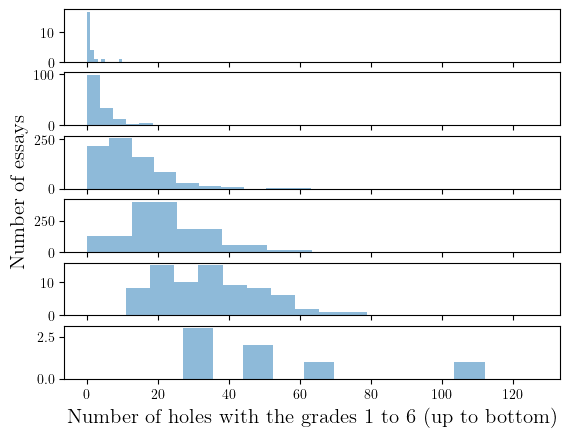
\includegraphics[width=8cm]{gradesh1.png}
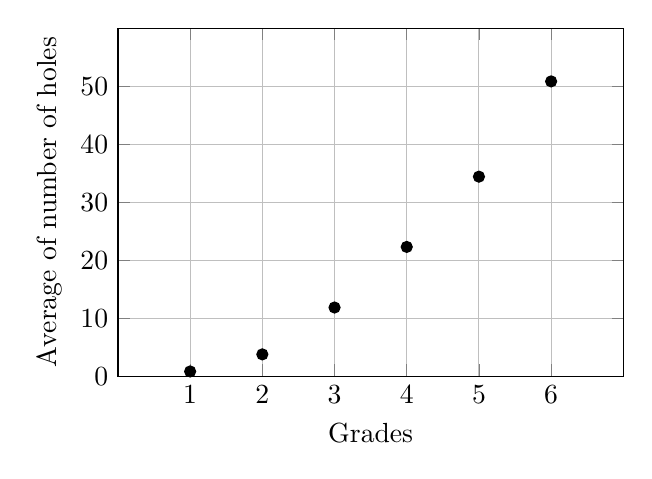
\begin{tikzpicture}
  \begin{axis}[
    xlabel={Grades},
    ylabel={Average of number of holes},
    grid=both,
    xmin=0,
    ymin=0,
    xmax=7,
    ymax=60,
    xtick={1,2,3,4,5,6},
    ytick={0,10,20,30,40,50},
    width=8cm,
    height=6cm,
    ]
    
    \addplot[only marks, mark=*, mark size=2pt] coordinates {
        (1, 0.8333333333333334)
        (2, 3.7777777777777777)
        (3, 11.857142857142858)
        (4, 22.308483290488432)
        (5, 34.42666666666667)
        (6, 50.857142857142854)
    };
  \end{axis}
\end{tikzpicture}
\caption{Number of holes increases as grade increases}
\label{fig:ds}
\end{figure}